\documentclass[11pt, oneside]{article}   	% use "amsart" instead of "article" for AMSLaTeX format
\usepackage{geometry}                		% See geometry.pdf to learn the layout options. There are lots.
\geometry{letterpaper}                   		% ... or a4paper or a5paper or ... 
%\geometry{landscape}                		% Activate for rotated page geometry
%\usepackage[parfill]{parskip}    		% Activate to begin paragraphs with an empty line rather than an indent
\usepackage{graphicx}				% Use pdf, png, jpg, or eps§ with pdflatex; use eps in DVI mode
								% TeX will automatically convert eps --> pdf in pdflatex		
\usepackage{amssymb, paralist}
\usepackage{verbatim}
\usepackage[utf8]{inputenc}
\usepackage{pmboxdraw}
\usepackage{listings}
\graphicspath{ {./images/} }

%SetFonts

\geometry{top=1.5cm}
\title{Shift Schedule Builder Desktop - Client Server}
\author{Yu-Chun Lin and Kuei-Ching Yang}
%\date{}							% Activate to display a given date or no date

\begin{document}
\maketitle
\section{Description}
Shift Schedule Builder Desktop is an application designed to simplify the task of shift arrangement for employees. Its primary aim is to provide a user-friendly interface that allows users to input their shift requirements and configurations easily and generate a shift that satisfies these shift requirements as much as possible.

The user can set up some basic shift parameters such as the number of days and the number of employees. The application will generate an empty shift that satisfies the basic requirement. In addition to basic shift parameters, users are able to add some shift requirements. The application provides several common shift requirements. For example, users are able to set up the expected number of working days in the given range of the shift. The application will automatically generate a schedule for them based on the given data and constraints. Since the scheduling problem is a multi-objective optimization problem, the users have to specify the weight of each constraints. If the user values a shift requirement a lot, the user has to specify bigger weight on that shift requirement.

The project is developed using Python and PyQt.
\subsection{UI Sketch}
We developed the UI by using \textbf{PyQt}. We have set up the basic parameters such as the width and the height of the main window by using the \textbf{QtDesigner}. The user interface is designed by inheriting the \textbf{QWidget}.

\subsubsection{Login}
In the beginning, the user has to login. The login dialog inherits QDialog. The login window will collect the username and password of the user to check and set different user. The login dialog serves as a view and controller in the application. After collecting the user's information, it will send the information to the database adapter to check if the user exists or not.

\begin{figure}[h]
\centering
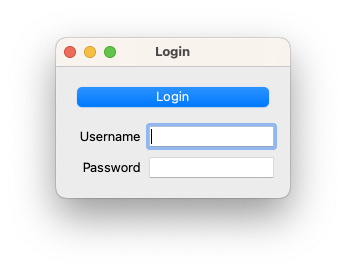
\includegraphics[scale=0.45]{login_window}
\caption{User Interface - Login Dialog}
\label{uilogin}
\end{figure}

\subsubsection{Main Window}
There is a class MainWindow which inherits QMainWindow and creates the frame of the window. The main window enables users to create multiple shifts by adding tabs and set up the parameters. The main window is composed of several components. The UI components are shown in the figure below. The detail of the design pattern will be elaborated in the architecture design section.
\begin{figure}[h]
\centering
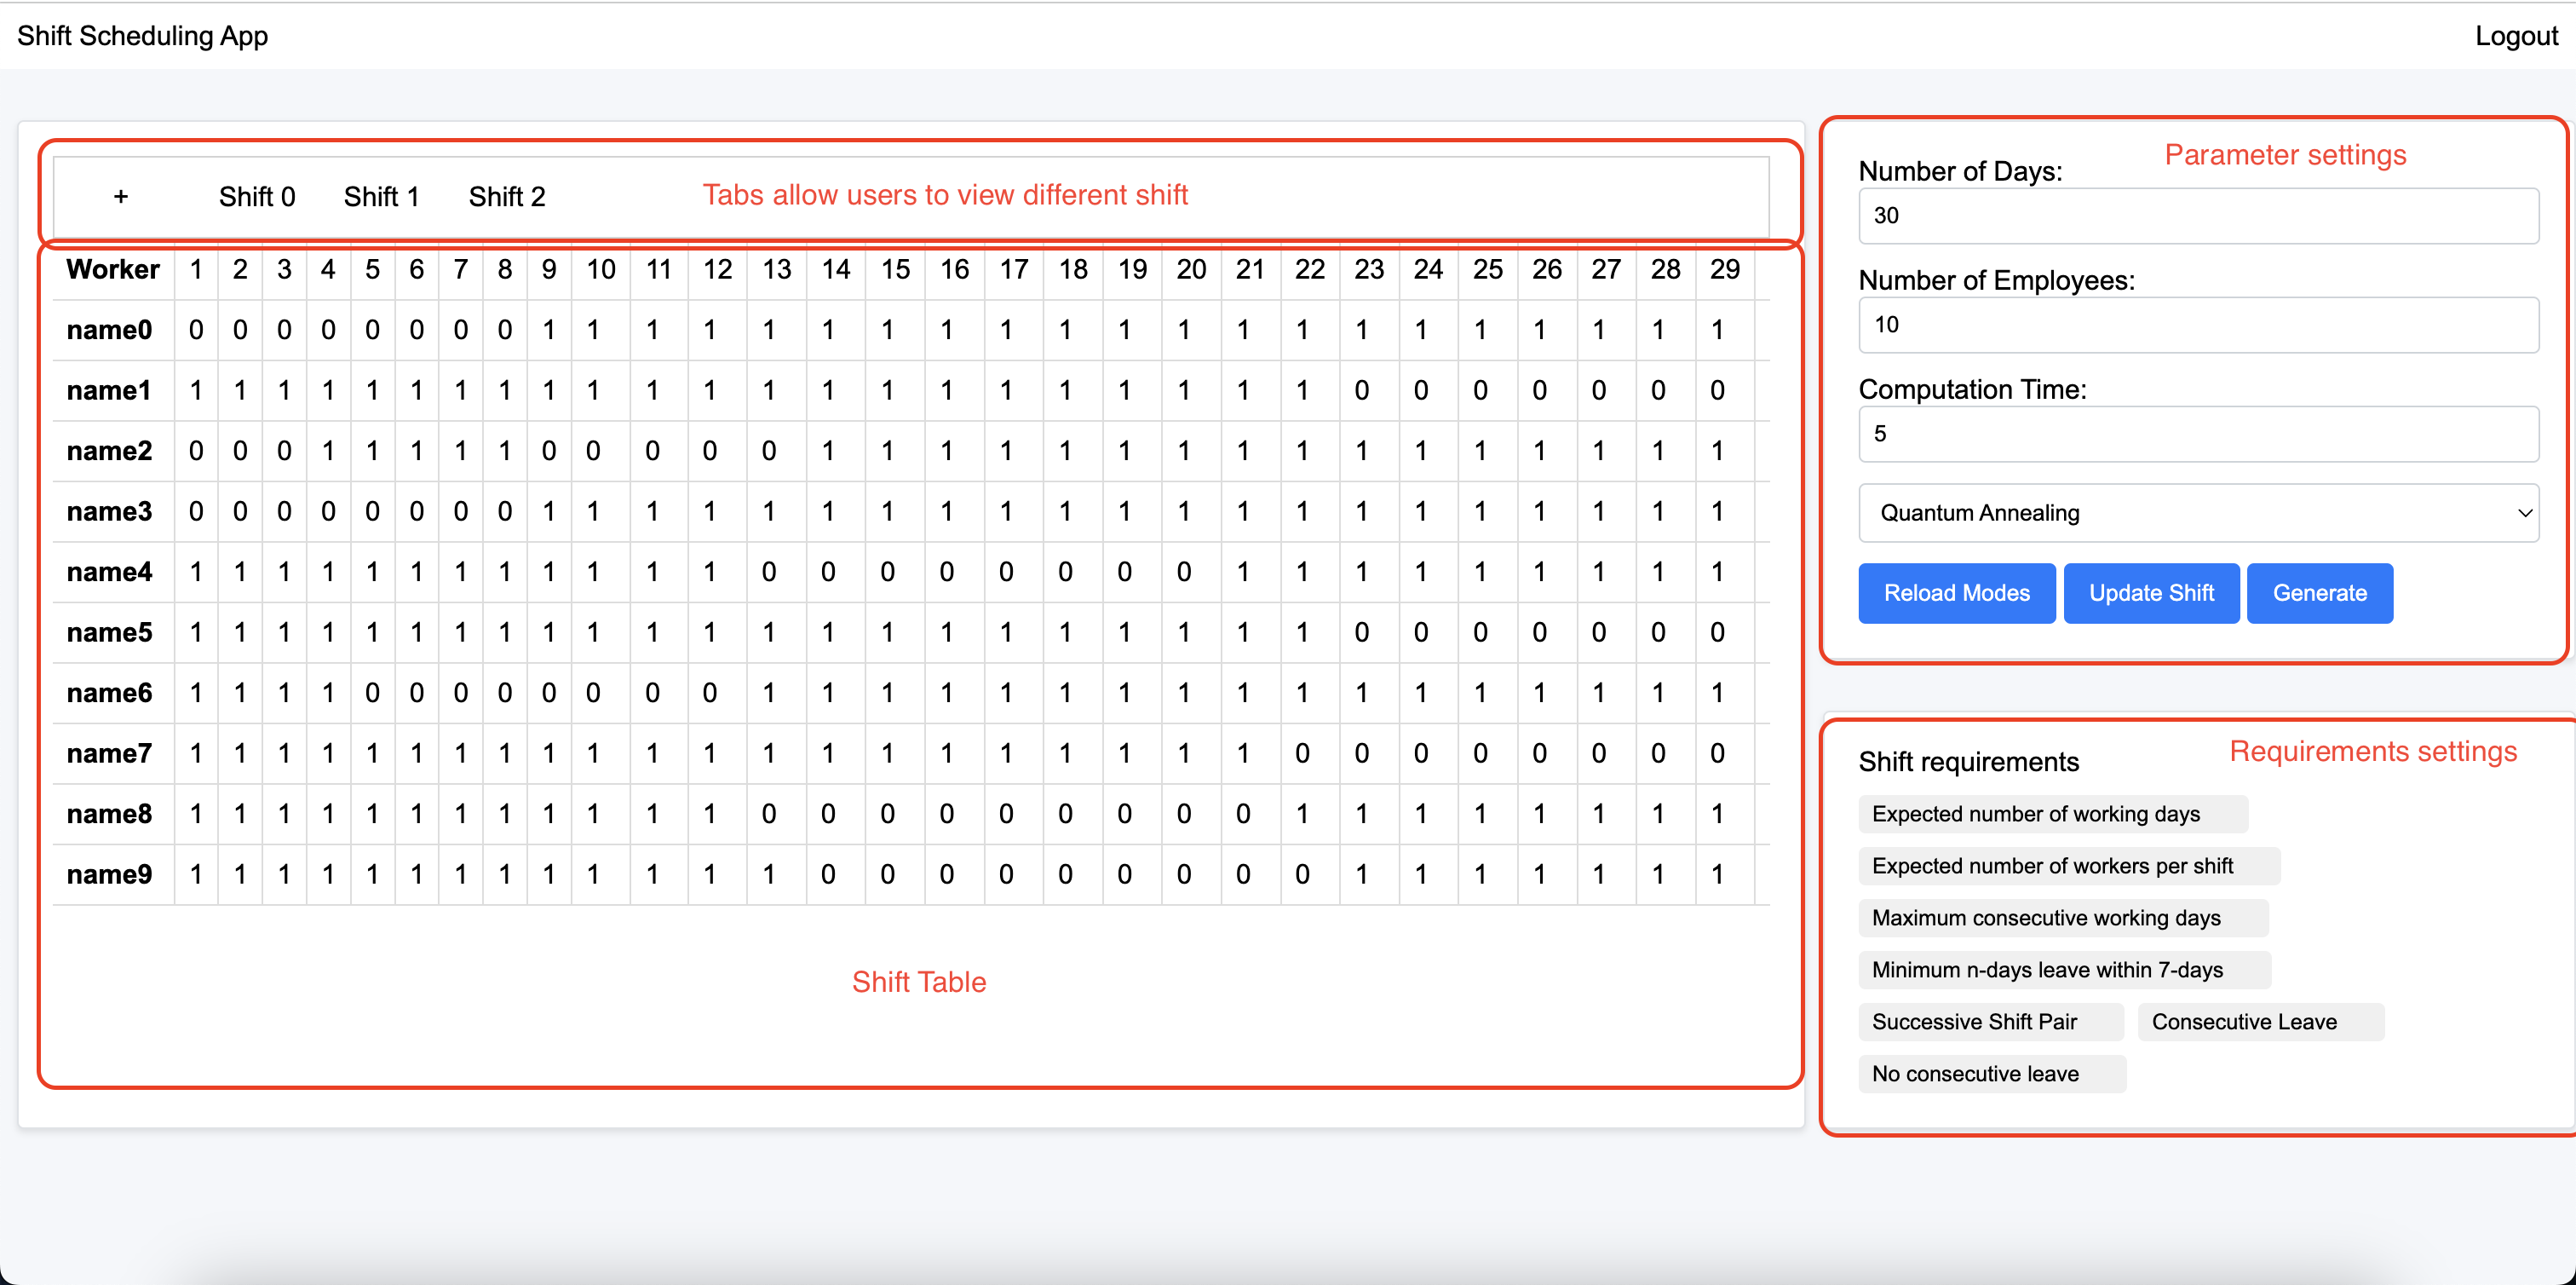
\includegraphics[width=\textwidth]{main_window}
\caption{User Interface - Main Window}
\label{uimainwindow}
\end{figure}

\iffalse
\begin{verbatim}
.
├── README.md
├── app.py
├── config.yml
├── requirements.txt
├── src
│   ├── algorithms
│   │    ...
│   ├── model
│   │   ...
│   ├── ui
│   │   ├── __init__.py
│   │   ├── form.ui
│   │   ├── login.py
│   │   ├── parameters_form.py
│   │   ├── shift_table.py
│   │   ├── table_widget.py
│   │   ├── tabs.py
│   │   ├── ui.py
│   │   ├── ui_form.py
│   │   └── working_area.py
│   └── utility
│       ├── ...
│       └── ...
└── unittests.py
\end{verbatim}
\fi

\subsection{Main use cases}

\subsubsection{Login}
\begin{description}
\item[Use case:] Login
\item[Actor:] System user
\item[Goal:] To login the system
\item[Overview:] When the users open the application, they have to sign in the system. 
If they type their username and password correctly, they are able to sign in. 
However, if they type either username or password wrong, the system will pop up a window showing a message that tells the users they failed to sign in.
\item[Actor action:]
\
\begin{enumerate}
\item user: A user types username and password
\item user: The user click login button
\item system: If both username and password are correct, then the system will allow user to login; otherwise, the system pop up a message that tells the user that the given information is not correct.
\item user: If the user is fail to login, the user may click the close button to close the application; otherwise, the system will close the login dialog window and show the application's user interface.
\end{enumerate}

\item[Alternative courses:]
\
\begin{description}
\item[Steps 1 and 2:] The user may click the close button to close the application.
\end{description}

\end{description}

\subsubsection{Sets up shift parameters}
\begin{description}
\item[Use case:] Sets up shift parameters
\item[Actor:] System user
\item[Goal:] To sets up shift parameters
\item[Overview:] Before the application generates a shift for the user, the user has to specify the shift paramters.
The parameters include days, number of workers, computation time, running mode.
\item[Actor action:]
\
\begin{enumerate}
\item user: A user types number of days in the parameters form.
\item system: The system regenerates a shift based on new parameter configuration.
\item user: The user types number of workers in the parameter form.
\item system: The system regenerates a shift based on new parameter configuration.
\item user: The user types the computation time in the parameter form.
\end{enumerate}

\item[Alternative courses:]
\
\begin{description}
\item[Steps 1 and 2:] The user may click the close button to close the application.
\end{description}

\end{description}

\subsubsection{Sets up shift requirements}
\begin{description}
\item[user case:] Setup shift requirements
\item[Actor:] System user
\item[Goal:]To sets up shift requirements
\item[Overview:] Before the application generates a shift for the user, the user is able to give some shift requirements.
The available shift requirements are the expected number of working days, the expected number of workers per shift, the successive shift pair, the consecutive 2 days off,  no more than consecutive days off, the maximum number of consecutive shifts, and the minimum number of N days off within 7 days.
\item[Actor action:]
\
\begin{enumerate}
\item user: The user click one of the shift requirements.
\item system: The system pops up a dialog to ask the user to provide the parameter of the shift requirement.
\item user: The user provides the preferred parameters.
\item user: The user click Add button to add the parameters.
\end{enumerate}

\item[Alternative courses]
\
\begin{description}
\item[Steps 3 and 4:] The user may click the close button to close the dialog.
\end{description}

\end{description}


\subsubsection{Generate a shift}
\begin{description}
\item[user case:] Generate a shift requirements
\item[Actor:] System user
\item[Goal:] To generate a shift
\item[Overview:]After the user finishes sets up the parameters and requirements, the user is ready to generate a shift. The user can click the run button to start generating the shift.
\item[Actor action:]
\
\begin{enumerate}
\item user: The user click the Run button to start generating a shift.
\item system: The run button becomes disabled and start generating a shift for the user.
\item system: The progress bar will keep posted the status of the task.
\item system: When finishing generating a shift, the system shows the shift on the user interface.
\item system: The run button will be unlocked so that users is able to re-run the task.
\end{enumerate}
\end{description}
%%%%
\subsubsection{Create a new shift}
\begin{description}
\item[user case:] Create a new shift
\item[Actor:] System user
\item[Goal:] To create a new shift
\item[Overview:] User can create a new shift by adding a tab. Each shift can be generated concurrently. 
\item[Actor action:]
\
\begin{enumerate}
\item user: The user click command+t on Mac computers or ctrl+t on windows computers.
\item system: The create a new tab for the user.
\end{enumerate}
\end{description}
%%%
\subsubsection{Save a shift}
\begin{description}
\item[user case:] Save a shift
\item[Actor:] System user
\item[Goal:] To save a shift
\item[Overview:]After acquiring a shift, the user is able to save his/her shift to the device.
\item[Actor action:]
\
\begin{enumerate}
\item user: The user click command+s on Mac computers or ctrl+s on windows computers.
\item system: The system pops up a window to ask the user to input the name of the shift and the location that the user wants to store the shift.
\item user: The user types the name and chooses a location.
\item system: The system exports the shift of the current tab to an excel sheet with given name and to the given location.
\end{enumerate}
\end{description}

\section{Database design}
The data models of the application are intricate. The database not only has to store the user’s information but also the shift data. Since users are allowed to set up multiple shift requirements, the number of the shift constraints will vary. Besides, the data size of the shift will vary based on the number of days and the number of  workers. It is intuitive to use the NoSQL database to store and load the data; thus, we choose MongoDB to store the data. The document and the data model of the application are compatible. In the database, we create two collections to store documents, one collection is Users and the other is Shifts. The entity relationship diagram is shown below.


\begin{figure}[h]
\centering
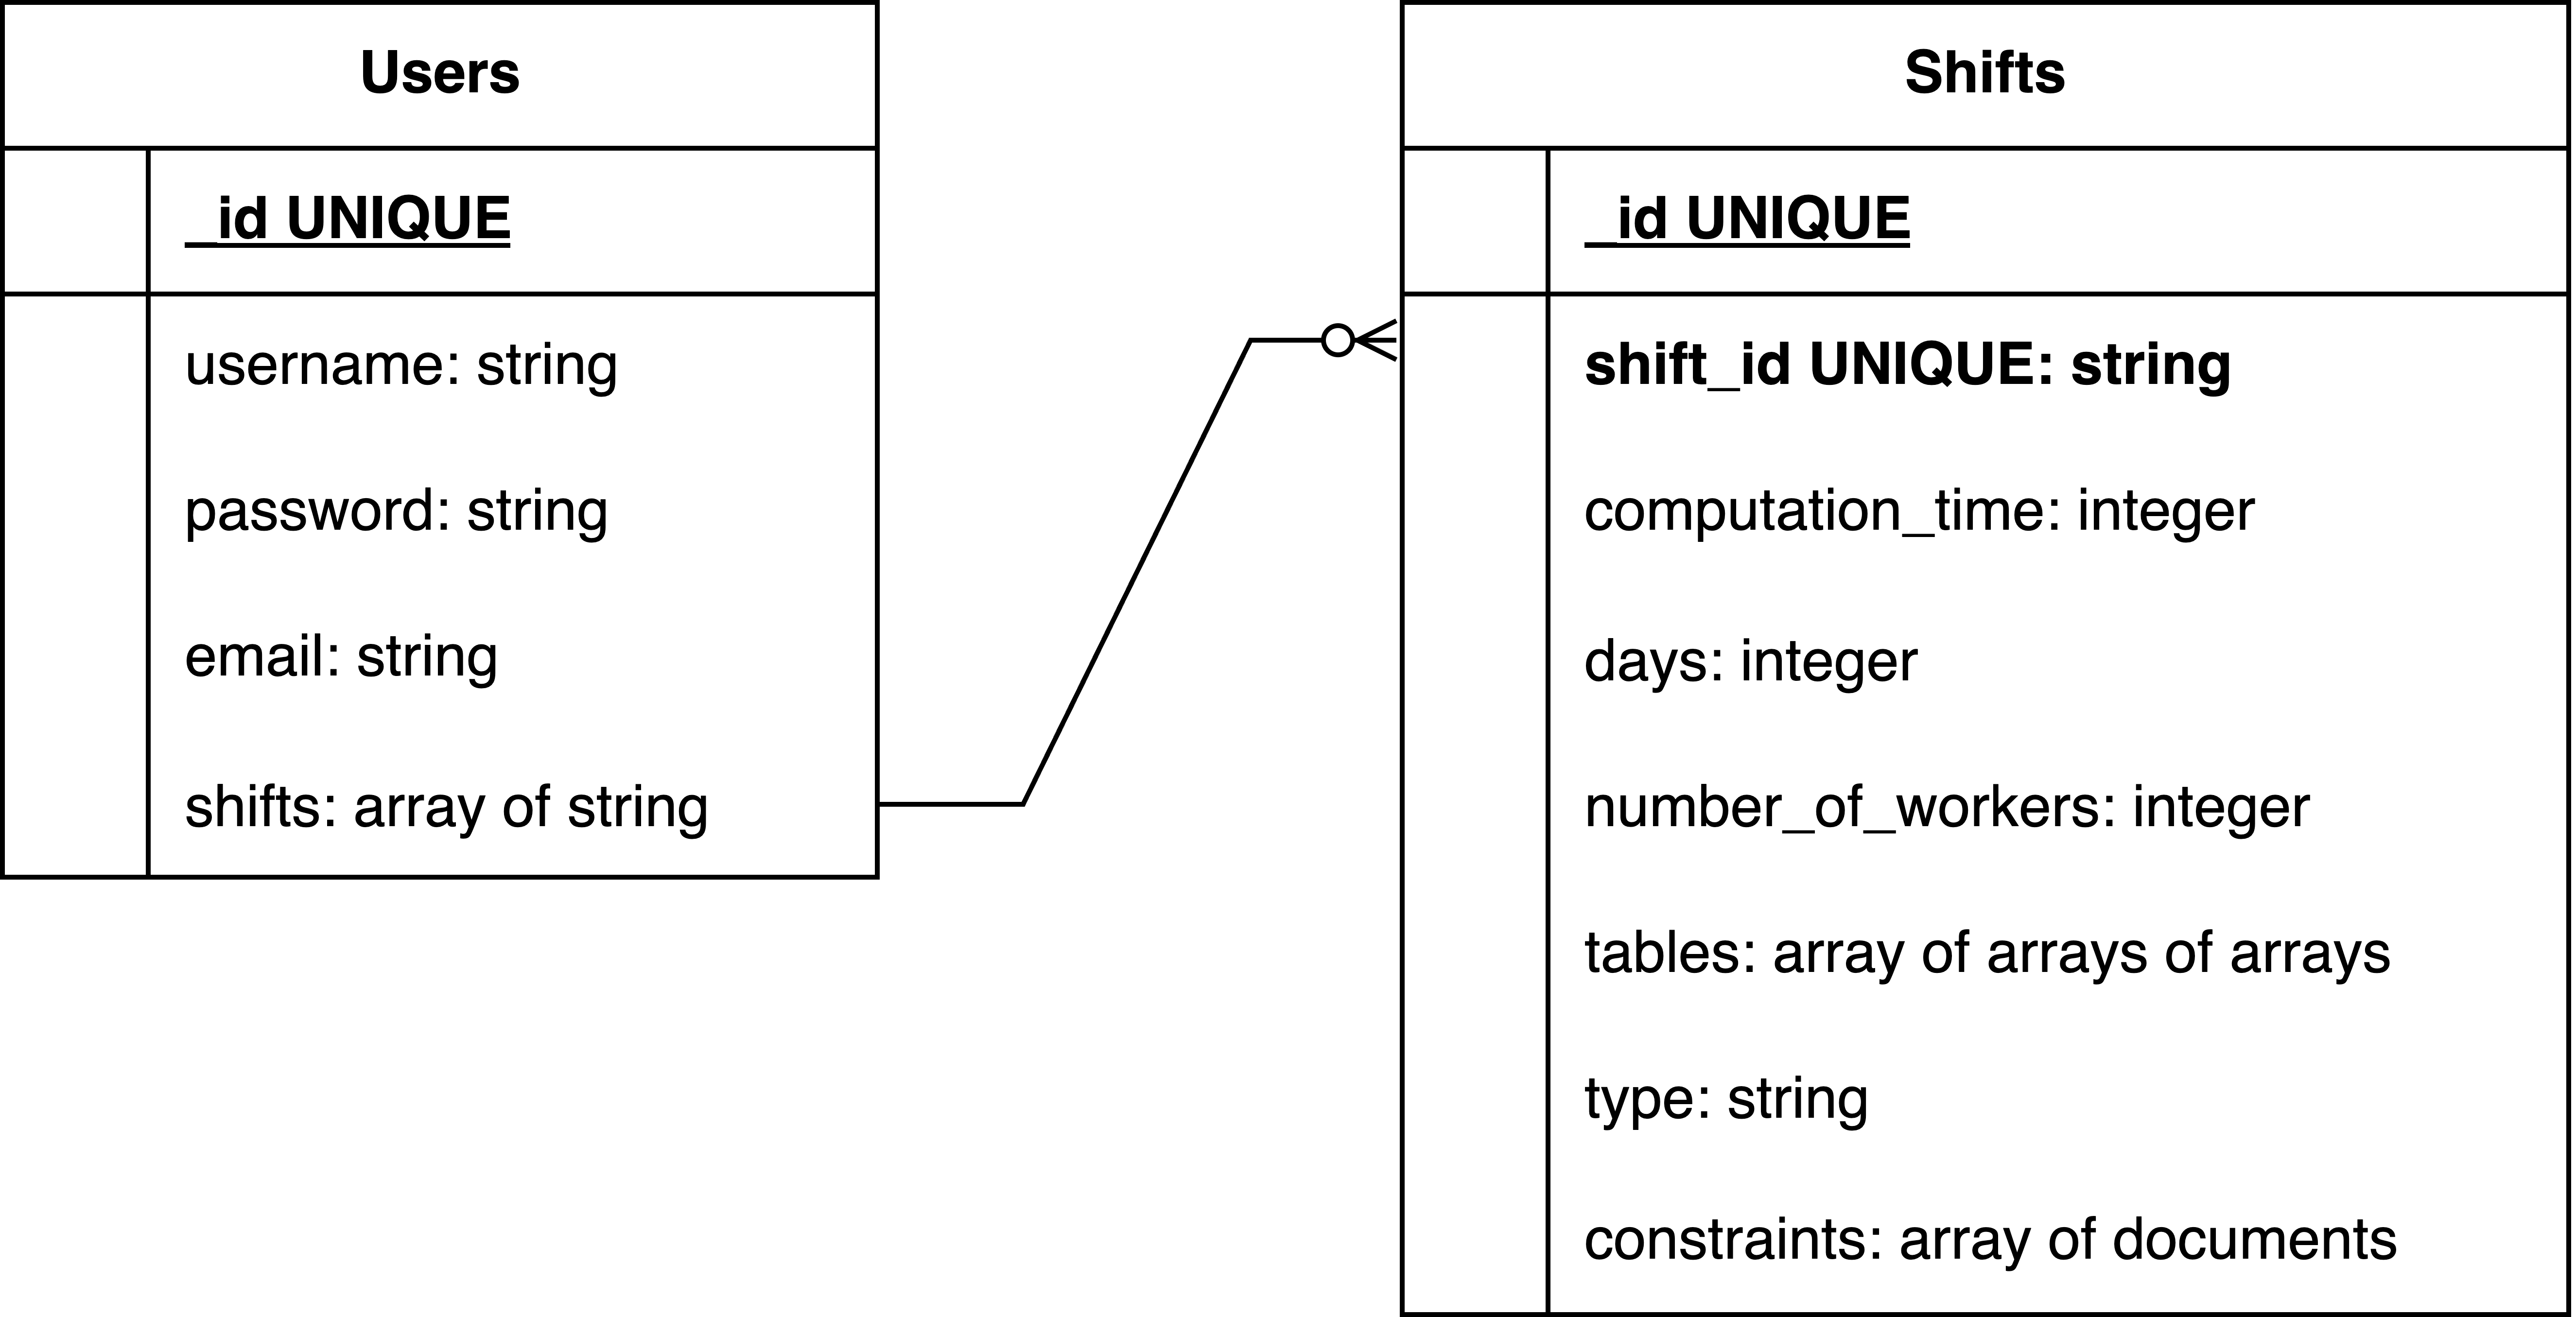
\includegraphics[width=\textwidth]{ erd }
\caption{Entity Relationship Diagram}
\label{erd}
\end{figure}


\subsection{Users}
The collection stores the basic information of a user such as username, password, email, and shifts. Here provides an example of a document. (In this prototype, we didn't use hash function to hash the password, but in the future, this feature will be added to protect user's information.)

\begin{verbatim}
[
  {
    _id: ObjectId("6518396323c0f9910c4fc915"),
    username: 'admin',
    password: 'password',
    email: 'email@gmail.com',
    shifts: [
      '66d74521-6947-4cd3-b2e9-d201140893bb',
      '0926ea12-8907-43e7-a2cb-340043eb7c12',
      '9223cea4-69f8-4dab-8832-4b48c952d91d',
      '0750a390-7f19-4341-9aa2-f41ccfc2c0f9'
    ]
  }
]
\end{verbatim}
The description of those fields is as follows.
\begin{compactenum}[1.]
\item \_id: A unique object id which is automatically generated by the database.
\item username : The username of the user.
\item password: The password of the user.
\item email: The email of the user.
\item shifts: A nested document that stores the shift ids owned by the user. In this example, the user owns 4 shifts. The shifts id will be used to load the shifts in Shifts collection.
\end{compactenum}

\subsection{Shifts}
The collection stores shifts' information. The shifts' information includes shift\_id, parameters, and the content of the shift. Here provides a snippet of a document in the collection.
\begin{verbatim}
[
  {
    _id: ObjectId("6519d6a87b2c1ef5a957ae5c"),
    shift_id: '594f91af-cade-47f3-aeff-a0d461285e1a',
    computation_time: 30,
    constraints: [
      {
        name: 'expected_number_of_working_days',
        parameters: { weight: '10', ewd: '20', days_off_index: [] }
      },
      {
        name: 'expected_number_of_workers_per_shift',
        parameters: { weight: '10', enwps: '8', days_off_index: [] }
      },
      {
        name: 'consecutive_2_days_leave',
        parameters: { weight: '10', days_off_index: [] }
      },
      {
        name: 'minimum_n_days_leave_within_7_days',
        parameters: { weight: '10', mndlw7d: '2', days_off_index: [] }
      }
    ],
    days: 30,
    name_list: [
      'name1', 'name2',
      'name3', 'name4',
      'name5', 'name6',
      'name7', 'name8',
      'name9', 'name10'
    ],
    number_of_workers: 10,
    tables: [
      [
        [
          1, 1, 1, 1, 0, 0, 1, 1, 1,
          1, 1, 0, 0, 1, 1, 1, 1, 1,
          1, 1, 0, 0, 0, 0, 0, 1, 1,
          1, 1, 1
        ],
        ...
        [
          1, 1, 0, 0, 1, 1, 1, 1, 1,
          1, 0, 0, 1, 1, 1, 1, 1, 0,
          0, 1, 1, 1, 1, 1, 1, 1, 1,
          0, 0, 0
        ]
      ],
      [
      	[
          1, 1, 1, 1, 0, 0, 1, 1, 1,
          1, 1, 0, 0, 1, 1, 1, 1, 1,
          1, 1, 0, 0, 0, 0, 0, 1, 1,
          1, 1, 1
        ],
        ...
        [
          1, 1, 0, 0, 1, 1, 1, 1, 1,
          1, 0, 0, 1, 1, 1, 1, 1, 0,
          0, 1, 1, 1, 1, 1, 1, 1, 1,
          0, 0, 1
        ]

      ]
    ],
    type: 'DAU'
  }
]
\end{verbatim}
\begin{compactenum}[1.]
\item \_id: A unique object id which is automatically generated by the database.
\item shift\_id: The id of the shift. The user entity will also store \textbf{shift\_id} in the \textbf{shifts} field.
\item computation\_time: The computation time of the shift.
\item constraints: The shift requirements. The field is a nested document that stores the name of the requirement and parameters.
\item days: The number of days
\item name\_list : The name list.
\item number\_of\_workers: The number of workers in the shift.
\item tables: Tables is a 3-D array which can stores multiple shifts. Each shift is a 2-D array.
\item type: The type of optimizer that solves the shift scheduling optimization problem. The type field will either be 'SA' or 'DAU'. SA means the optimization algorithm is simulated annealing algorithm, and DAU means the problem is solved by using the digital annealing unit.
\end{compactenum}

\subsection{Sample Code}

Since we use NoSQL database, we are only able to provide the sample code that we used to insert, search, and  update the document.
The following code snippets are parts of class DataAdapter.

\subsubsection{Search user}
\begin{verbatim}
user_data = self.db.Users.find_one({"username": username, "password": password})
\end{verbatim}

\subsubsection{Update user's shifts}
The following code snippet update user's shifts by using update\_one function.
\begin{verbatim}
user_collection = self.db.Users
user_collection.update_one(
	{"username": user.getUsername()}, 
	{"$set": {"shifts": user.getShifts()}}
)
\end{verbatim}

\subsubsection{Save a shift}
The following code snippet uses update\_one to save a shifts, but we set upsert=True for the case that the shift doesn't originally exist. In that case, it will insert a document.
\begin{verbatim}
collection = self.db.Shifts
inserted_data = shift.getShiftConfiguration() 
inserted_data['table'] = tables
collection.update_one({"shift_id" : shift.getShiftId()}, {"$set": inserted_data}, upsert=True)
\end{verbatim}

\subsubsection{Load a shift}
The following code snippet will find a shift based on given shift\_id.
\begin{verbatim}
shift = self.db.Shifts.find_one({"shift_id": shift_id})
\end{verbatim}

\section{Architectural design}
The scope of the application includes the user interface, server, database, and solvers. The user interface collects user's preference of the shift. The server components processes user's requests to load/save the data and handle the computation. The database stores and loads the users' information and shifts. Solvers are used to solve the optimization problem to generate the shift that satisfies the requirements as much as possible. After acquiring the solution from cloud computation or on-device computation, Solvers will return the shift back to view/controller to show on the user interface. In this version, solvers will use web socket to do the communication. After View/controller received the shift data, it will send the data back to server to store the data into the database. 

The following section will give details on architecture design for each component.

\begin{figure}[h]
\centering
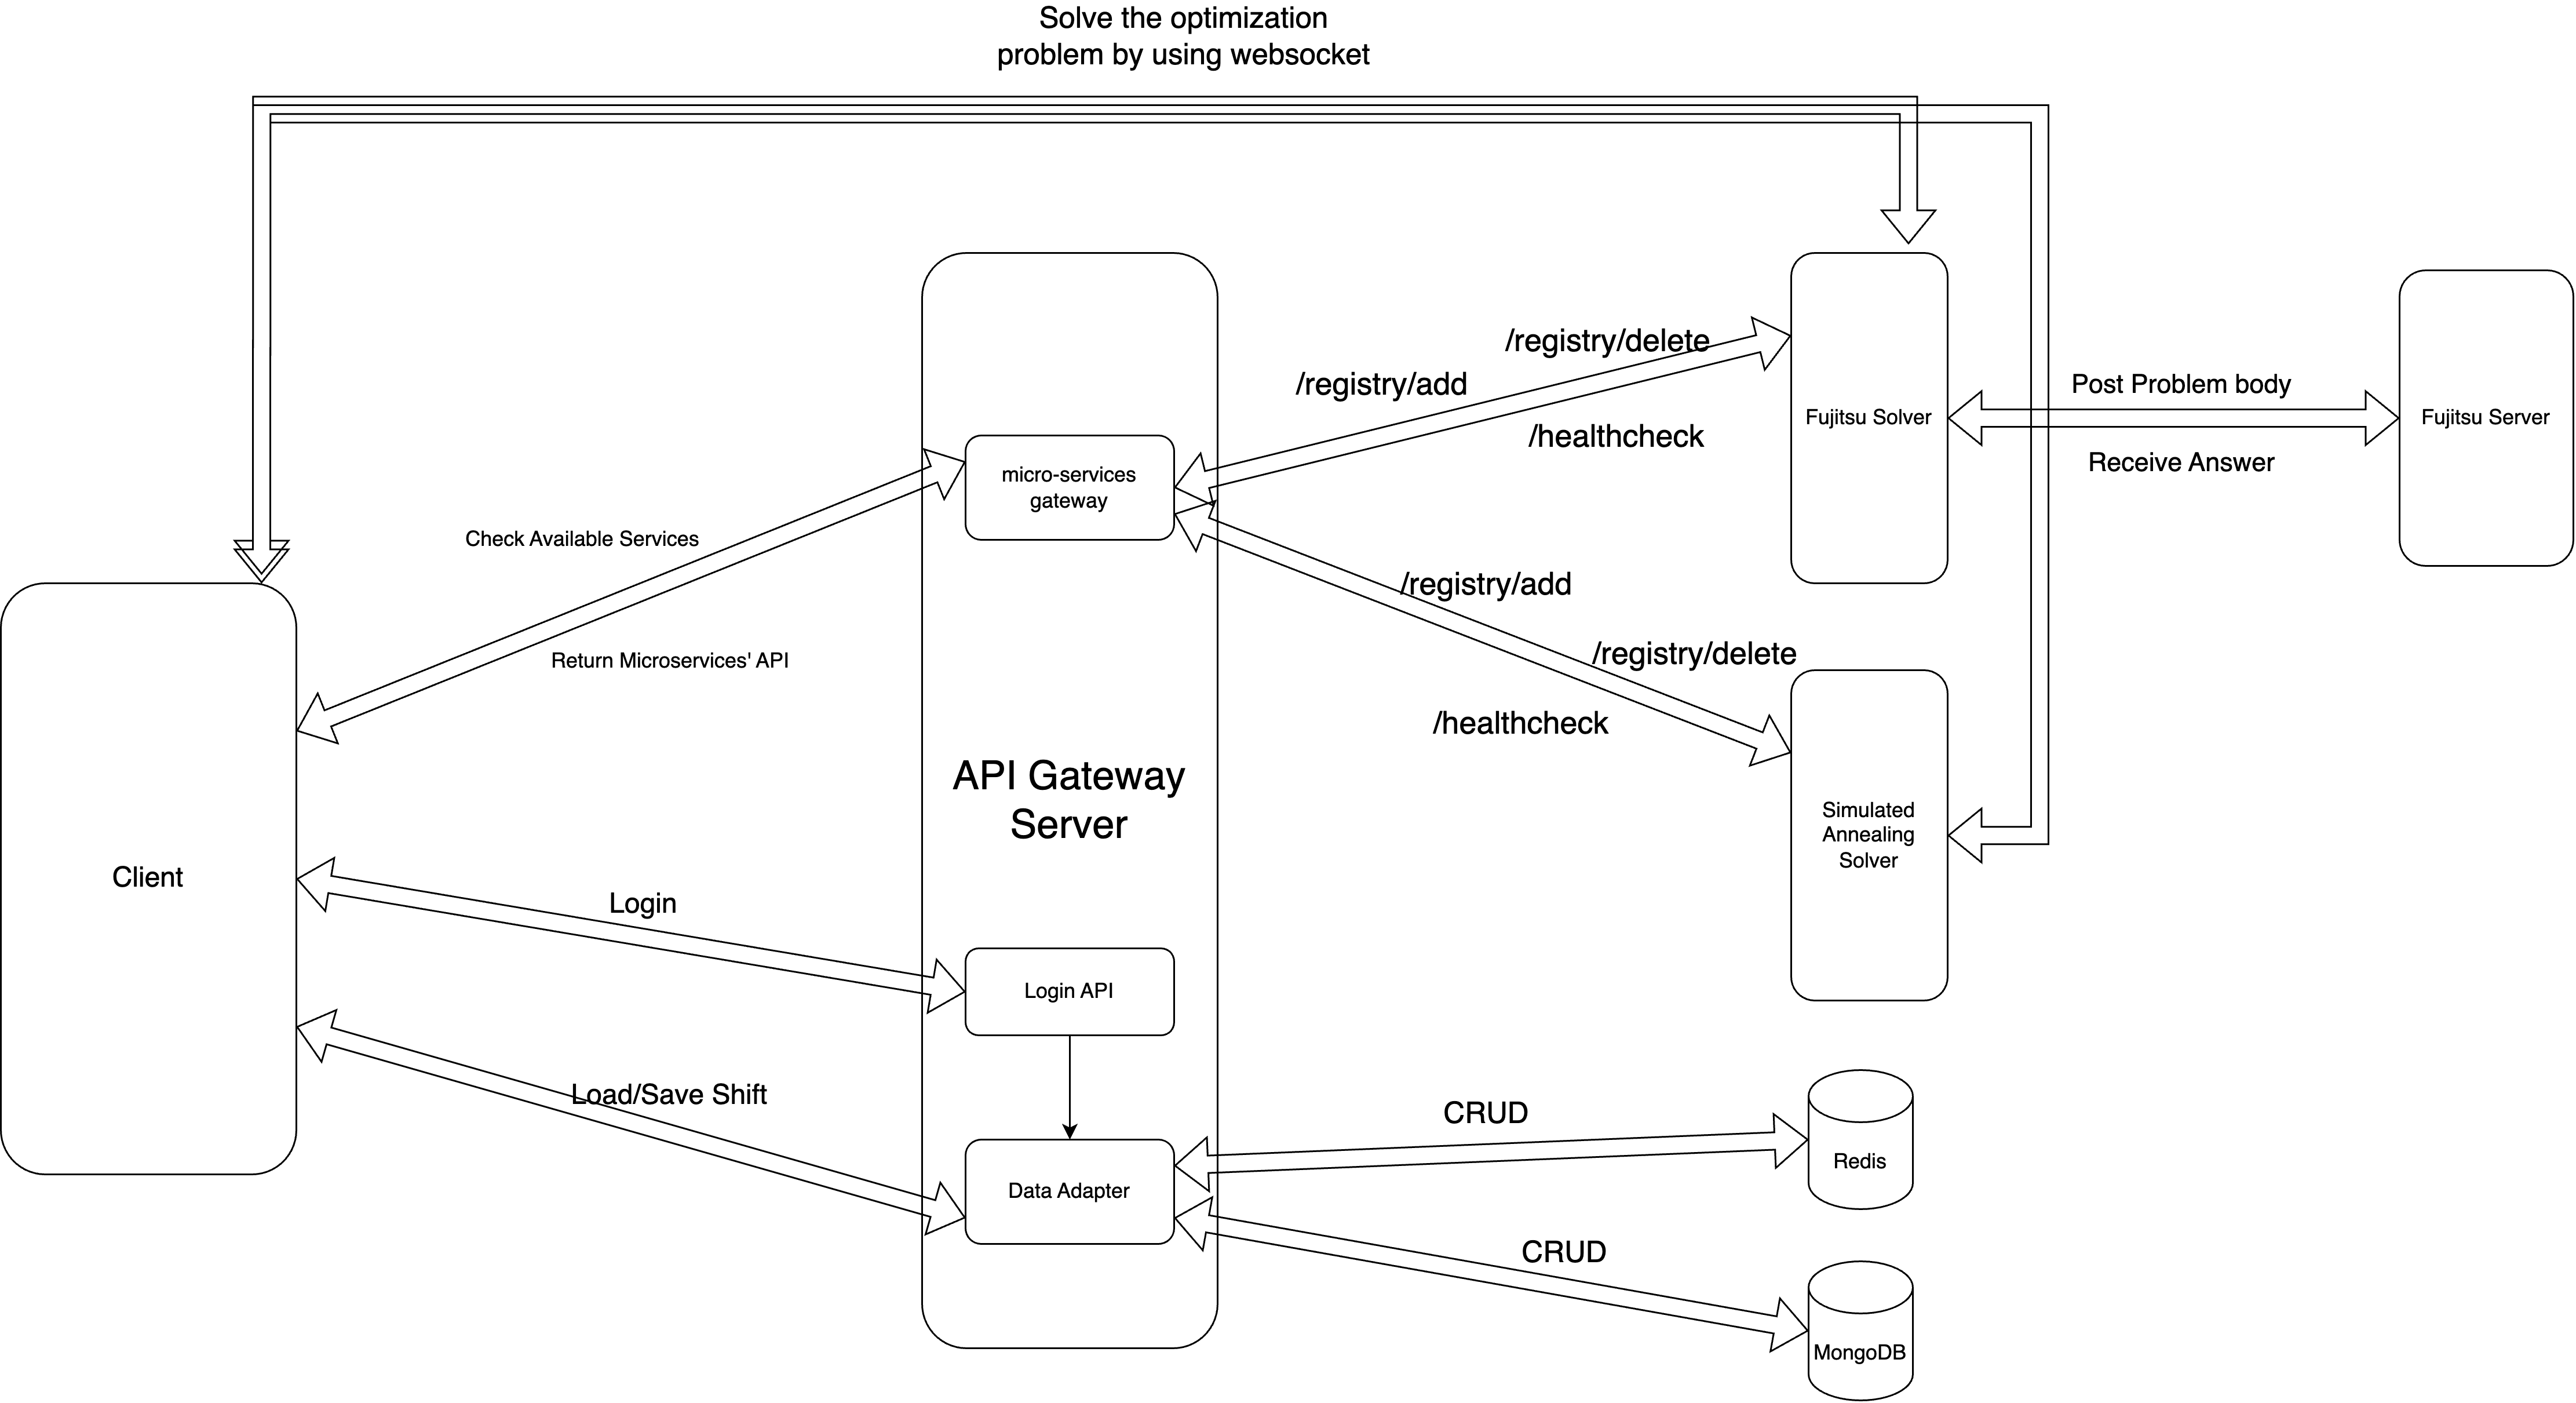
\includegraphics[width=\textwidth]{arch1}
\caption{System Architecture}
\label{sysarch}
\end{figure}

\subsection{Server}
We developed a tiny framework that enables us to flexibly extend the function of the server. The server's architecture is as shown in Fig.~\ref{framework}
The server is composed of two parts, a http server and a web socket server. When the server received an incoming request, the instance of \textbf{ProtocolTypeRouter} will do routing based on the request's protocol. For example, if the request is a http request, ProtocolTypeRouter will transfer the request to HttpServer. When the server received a request sent from ProtocolTypeRouter, both servers will do routing based on the request's URI to a certain route. Each route will handle the request and the response. The only things that developers have to do is to define the API endpoints and override the handle function of the corresponding Route to handle the request.
Here provides a snippet of code that shows how to use this tiny framework.
\begin{verbatim}
class TestRoute(Route):

    def handle(self):
        data = {
            "message": "successful"
        }
        self.response.send(200, json.dumps(data), content_type="application/json")


class EchoWebsocketRoute(WebSocketRoute):

    def handle(self):
        while True:
            received_message = self._recv()
            print("Received Text: ", received_message)
            if received_message is None:
                break
            else:
                self.response.send(received_message)
                
if __name__ == '__main__':
    server = ProtocolTypeRouter({
        'http': HttpServer(routes=[(r'/', TestRoute)]),
        'websocket': WebSocketServer(routes=[(r'/chat', EchoWebsocketRoute)])
    })
    server.run()
\end{verbatim}
We just need to inherit Route type and override handle function, and  register the Route type to the corresponding server and specify the uri.
This enables us to easily extend the function of server. Fig.~\ref{serveruml} details the UML of the server side.

\begin{figure}[h]
\centering
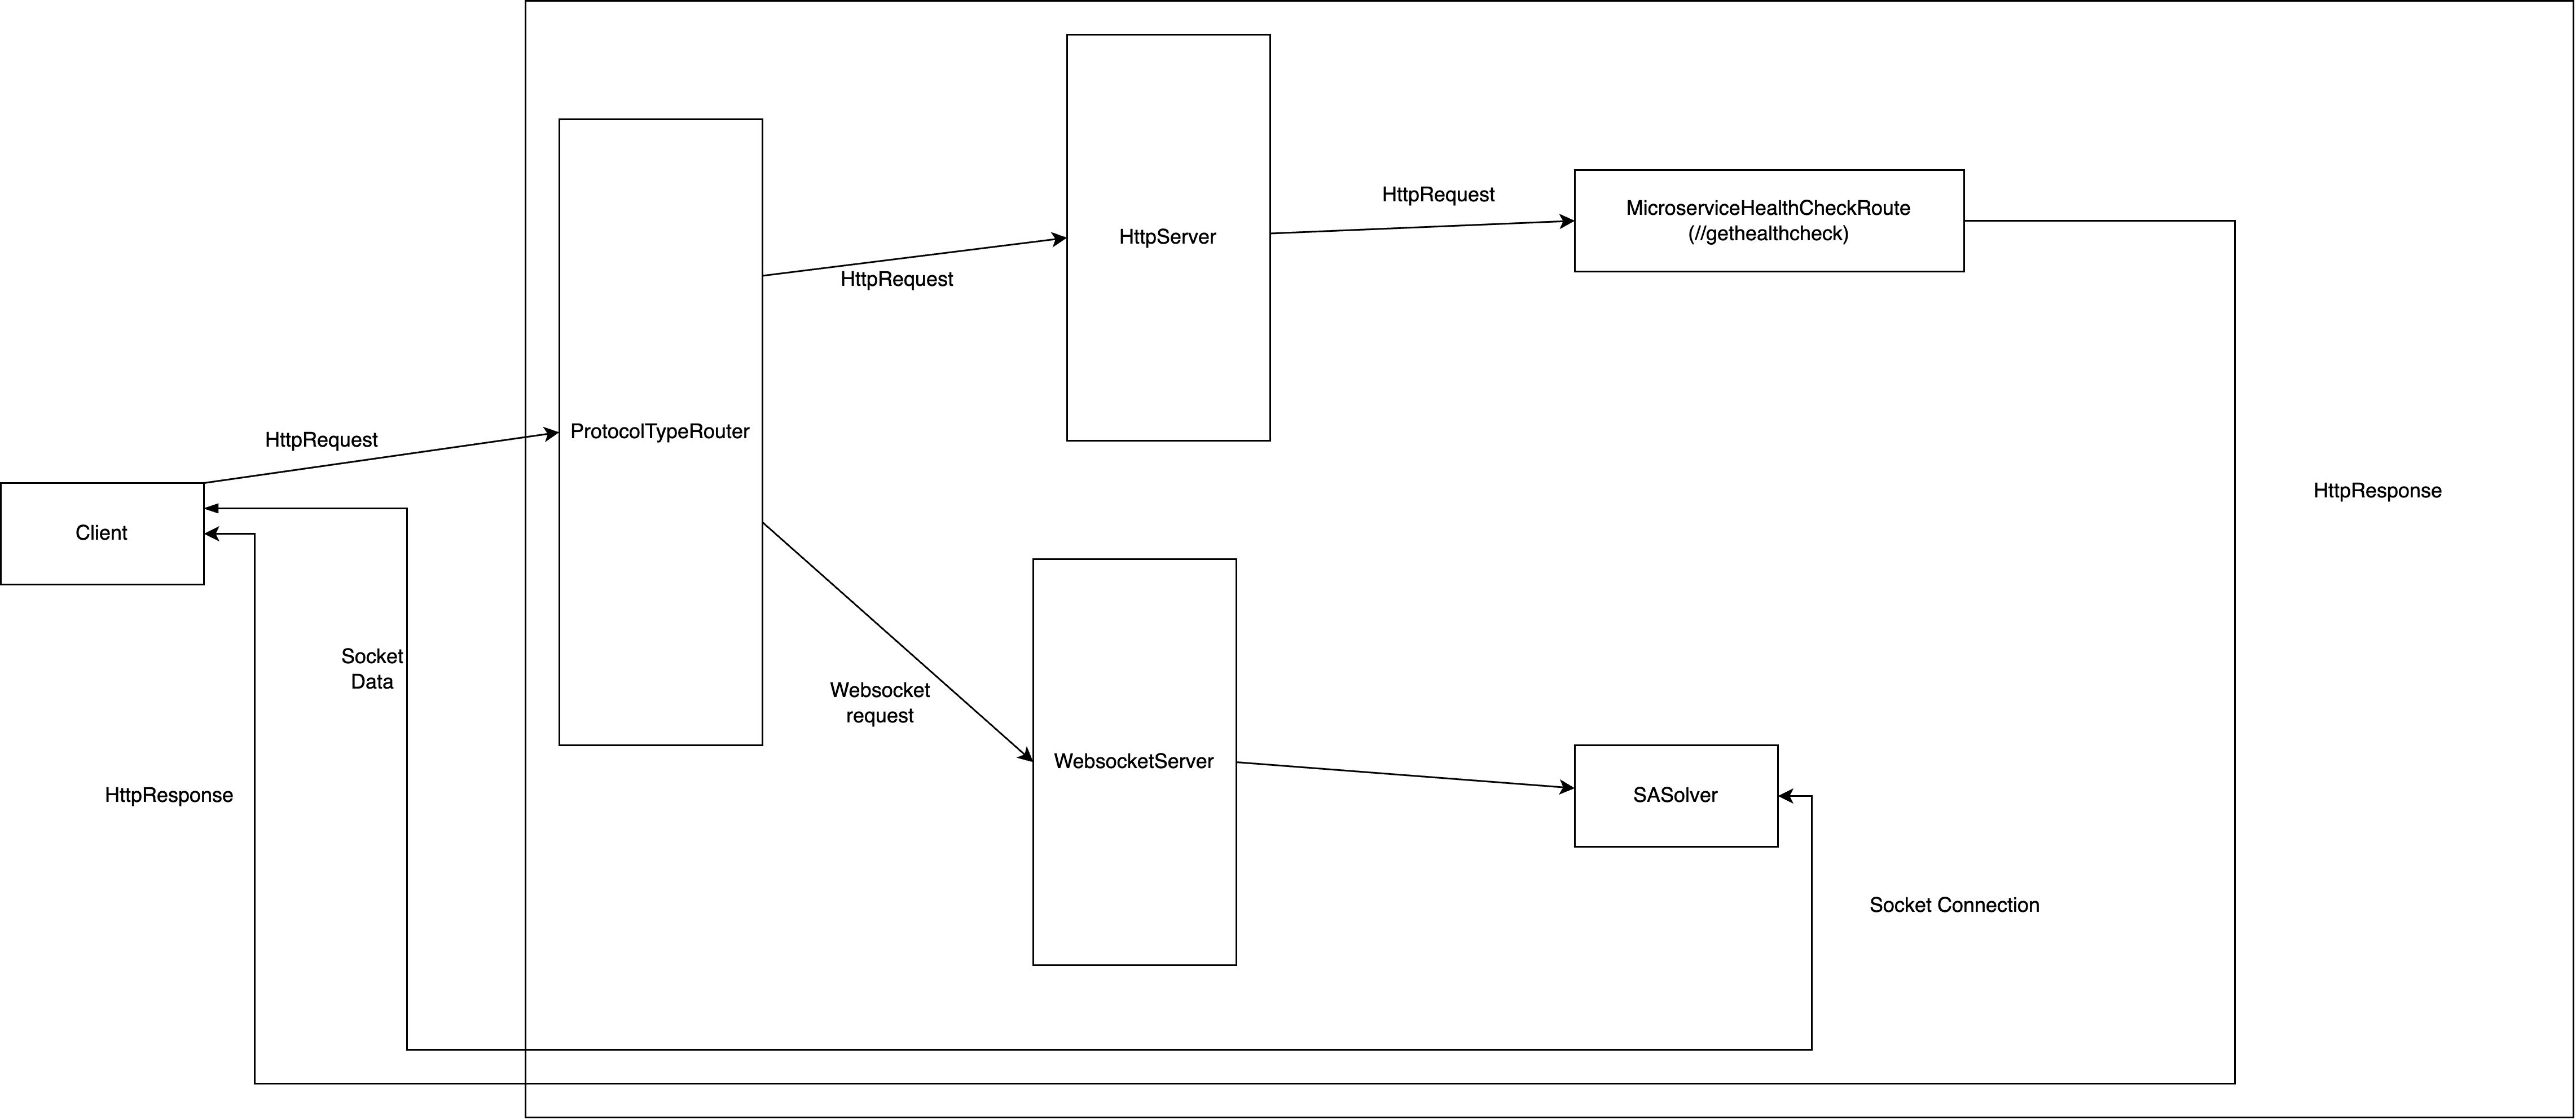
\includegraphics[width=\textwidth]{framework}
\caption{The architecture of the tiny framework}
\label{framework}
\end{figure}

\begin{figure}[h]
\centering
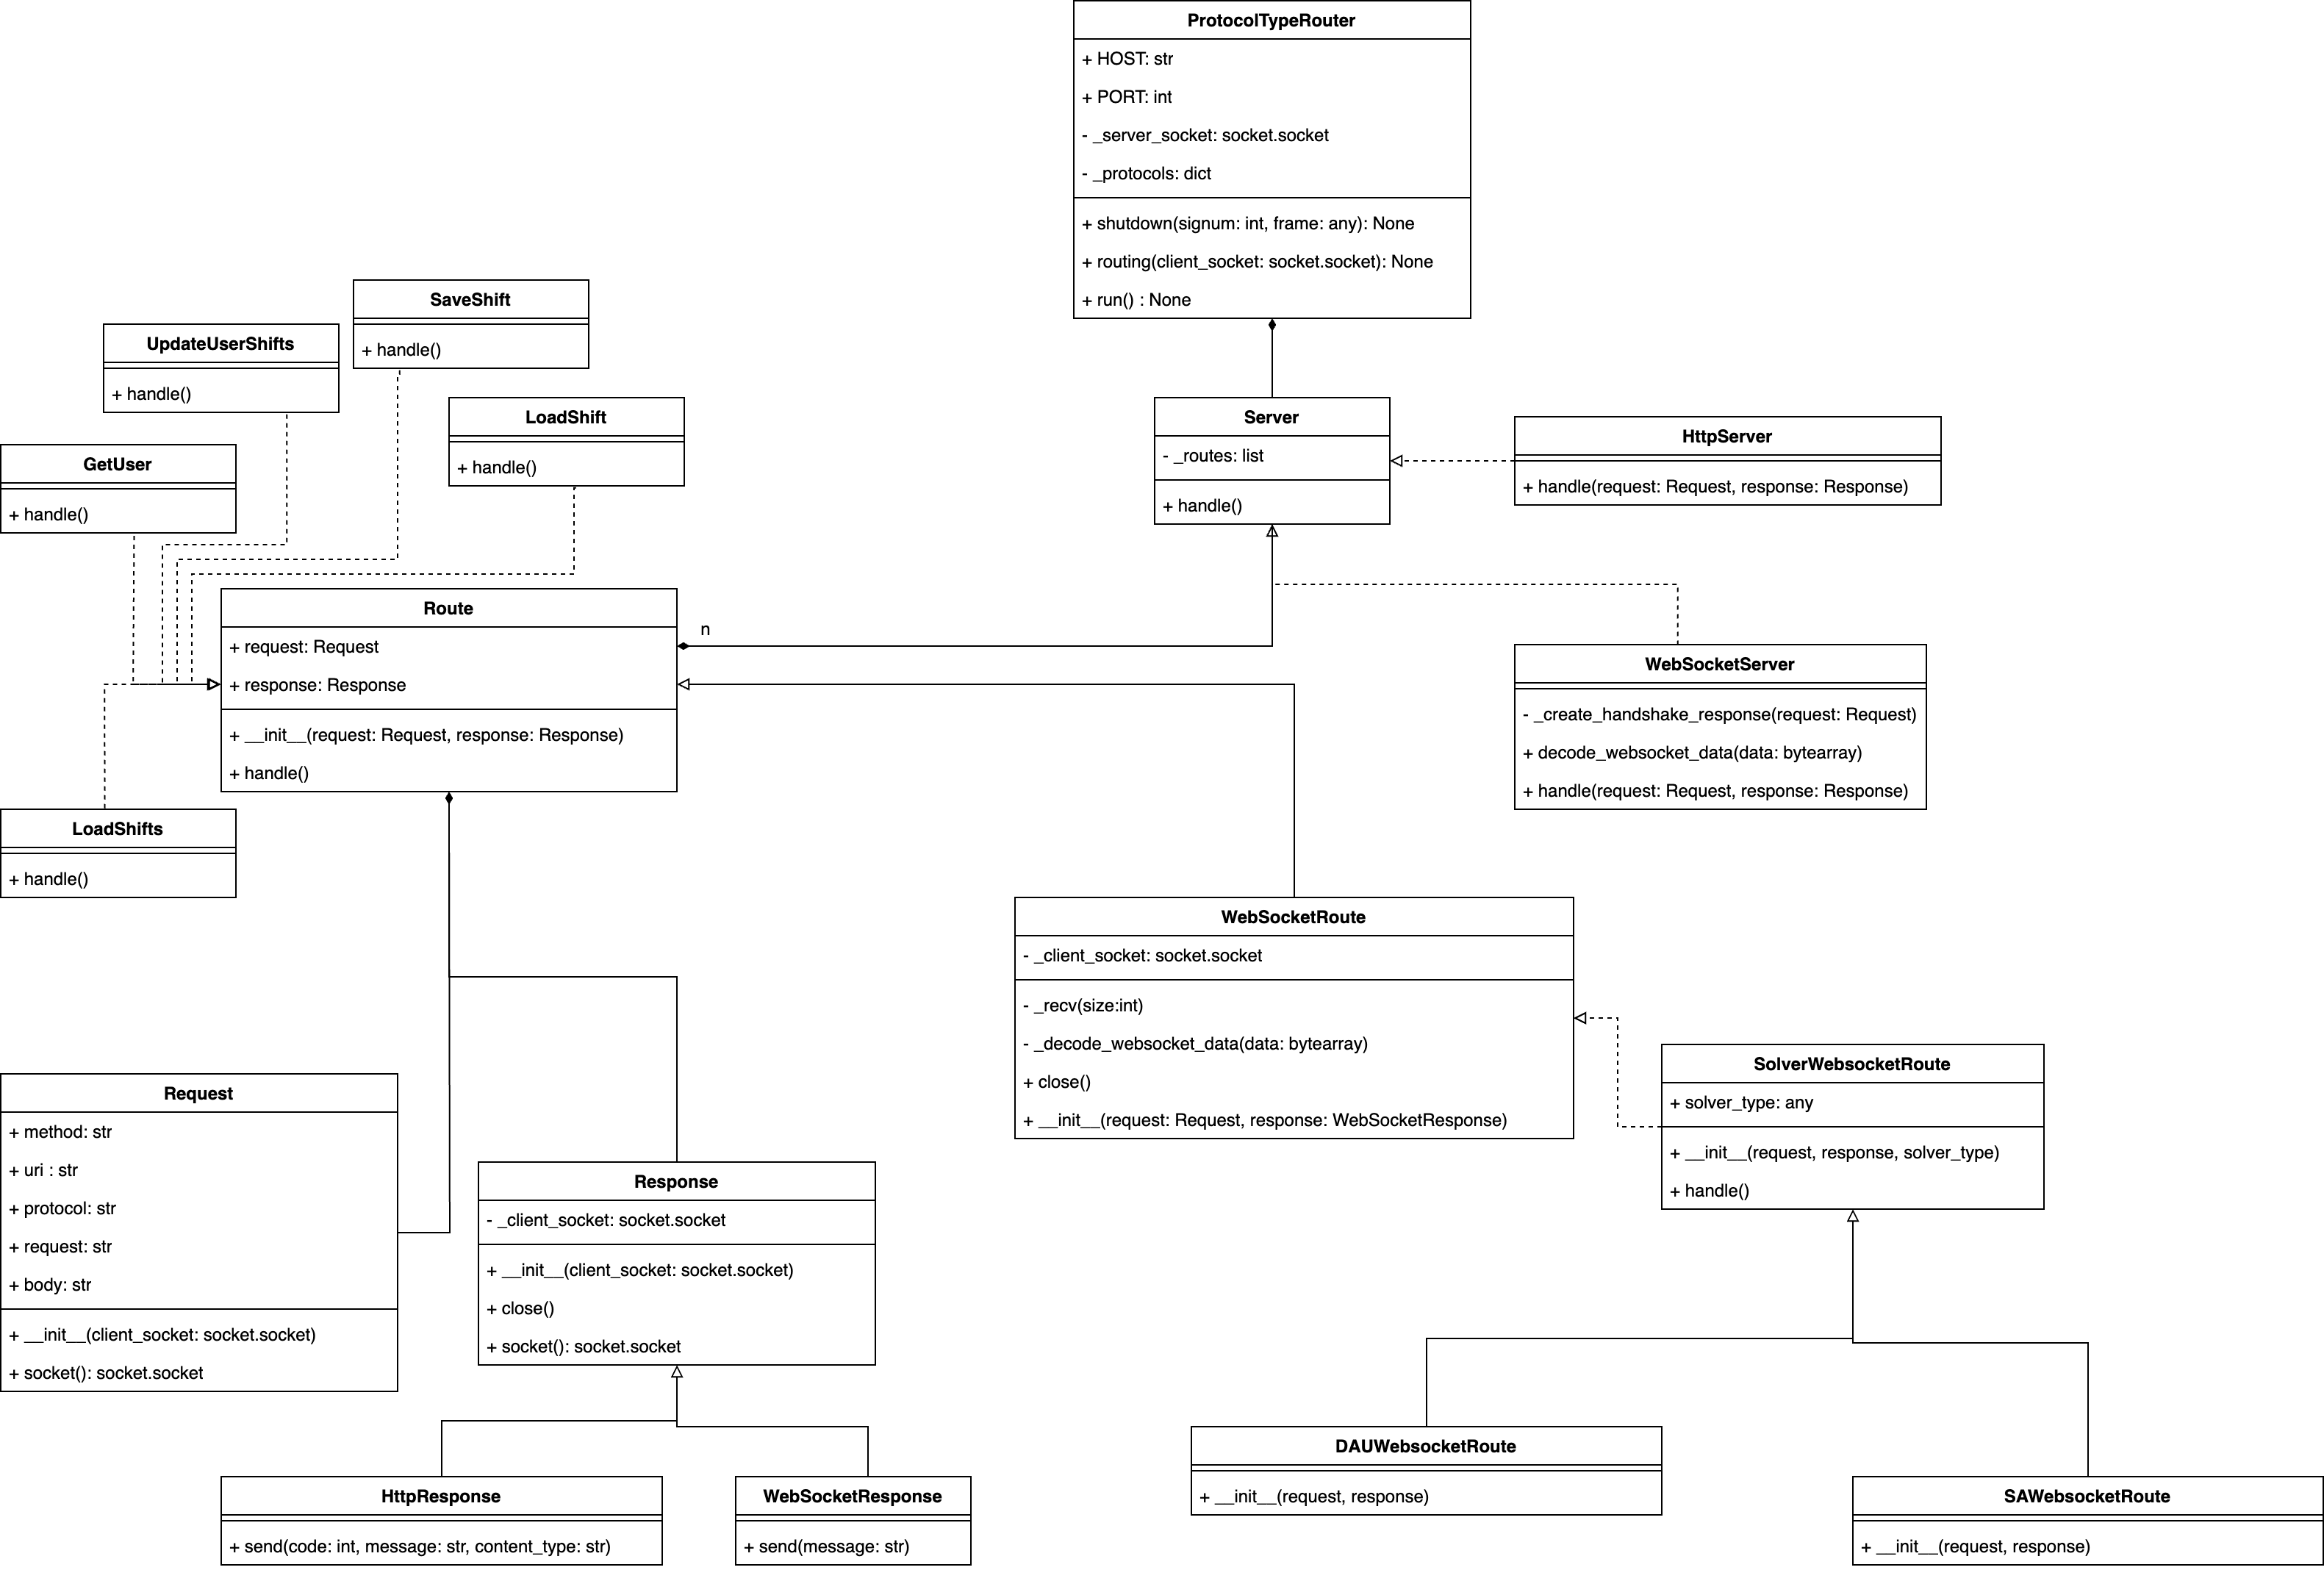
\includegraphics[width=\textwidth]{serverUML}
\caption{The UML diagram of the server}
\label{serveruml}
\end{figure}

\subsubsection{RemoteSolver}
RemoteSolver is a class that establishes the web socket connection between UI and the server. 
It also processes the message sent from the server side and connect itself and the progress bar to update the status.

We wrote two remote solvers, RemoteDAUSolver and RemoteSASolver. The corresponding APIs are ws://localhost:8888/dau and ws://localhost:8888/sa. Both solvers inherit from RemoteSolver.
When the function solve is called, it will use web socket to send the optimization problem to the server. Here provides a simple example of the data.
The data format in the communication is in the json format.
\begin{verbatim}
{
    "type": "SA",
    "days": 30,
    "number_of_workers": 10,
    "computation_time": 10000,
    "reserved_leave": [],
    "constraints": [
        {
            "name": "expected_number_of_working_days",
            "parameters": {
                "weight": "10",
                "ewd": "20"
            }
        },
        {
            "name": "expected_number_of_workers_per_shift",
            "parameters": {
                "weight": "8",
                "enwps": "8"
            }
        }
    ],
    "content": [
        {
            "name": "name1",
            "shift_array": ["0","0","1","1","0","0","1","1","1","1","1","0","0",
            "0","1","1","0","1","1","1","1","1","0","1","1","1","1","1","1","1"
            ]
        },
        {
            "name": "name2",
            "shift_array": [...]
        },
        ...
     ]
}

\end{verbatim}
In the server side, we defined a class SolverWebsocketRoute which inherits from WebSocketRoute. 
The class will process the request and invoke the corresponding computation service to do the optimization problem.
We also defined two classes that inherit from SolverWebsockeRoute, which are DAUWebsocketRoute and SAWebsocketRoute.
Both give the computation service to the base class.
During the computation, the server will keep UI posted the state of the computation. For example, when the problem is compiled. It will use web socket to send
\begin{verbatim}
{"message": "status", "status" : "compiling"}.
\end{verbatim}
The user interface can update the status of computation to the user.

\subsection{UI}
As shown in Fig.~\ref{uimainwindow}. The main window is composed of several UI components. The relationship between each component is presented in the Fig.~\ref{uiuml}.
\begin{figure}
\centering
\includegraphics[width=\textwidth]{ui_uml}
\caption{UI's UML}
\label{uiuml}
\end{figure}
\subsection{Solvers(Algorithms)}
The shift scheduling problem is modeled by the quadratic unconstrained binary optimization (QUBO) problem. 0 represents a day off and 1 represents a working day. Once the user adds shift requirements, they implicitly formulate their QUBO problem. The QUBO problem is compiled in user's computer and solved by either the digital annealer or the simulated annealing algorithm on users' device. After the device finishes computation, the solution is then post-processed to generate the final schedule. Digital annealer is a computation service provided by Fujitsu Ltd. Digital annealer is a quantum-inspired device that is good at solving optimization problems.

In this prototype, the application offers limited shift requirements for users to choose from. The available shift requirements are listed and explained in detail below. The source code of the mathematic constraints is written in this file constraints.py.

Each constraint in the project represents a class. The constraint inherits a base class which is defined as follows:
\begin{verbatim}
class ConstraintFunction(object):
    
    def __init__(self, X:Array, **kwargs):
        self._X = X
        self._weight = float(kwargs['weight'])
        
    def hamiltonian(self) -> Model:
        pass

    def weighted_hamiltonian(self) -> Model:
        return self._weight * self.hamiltonian()
    
    def evaluate(self, table) -> dict:
        pass
\end{verbatim}

In the project, there are two solvers available. One is digital annealer, and the other is simulated annealing solver. The UML digram is shown in Fig.~\ref{umlsolvers}.

\begin{figure}[h]
\centering
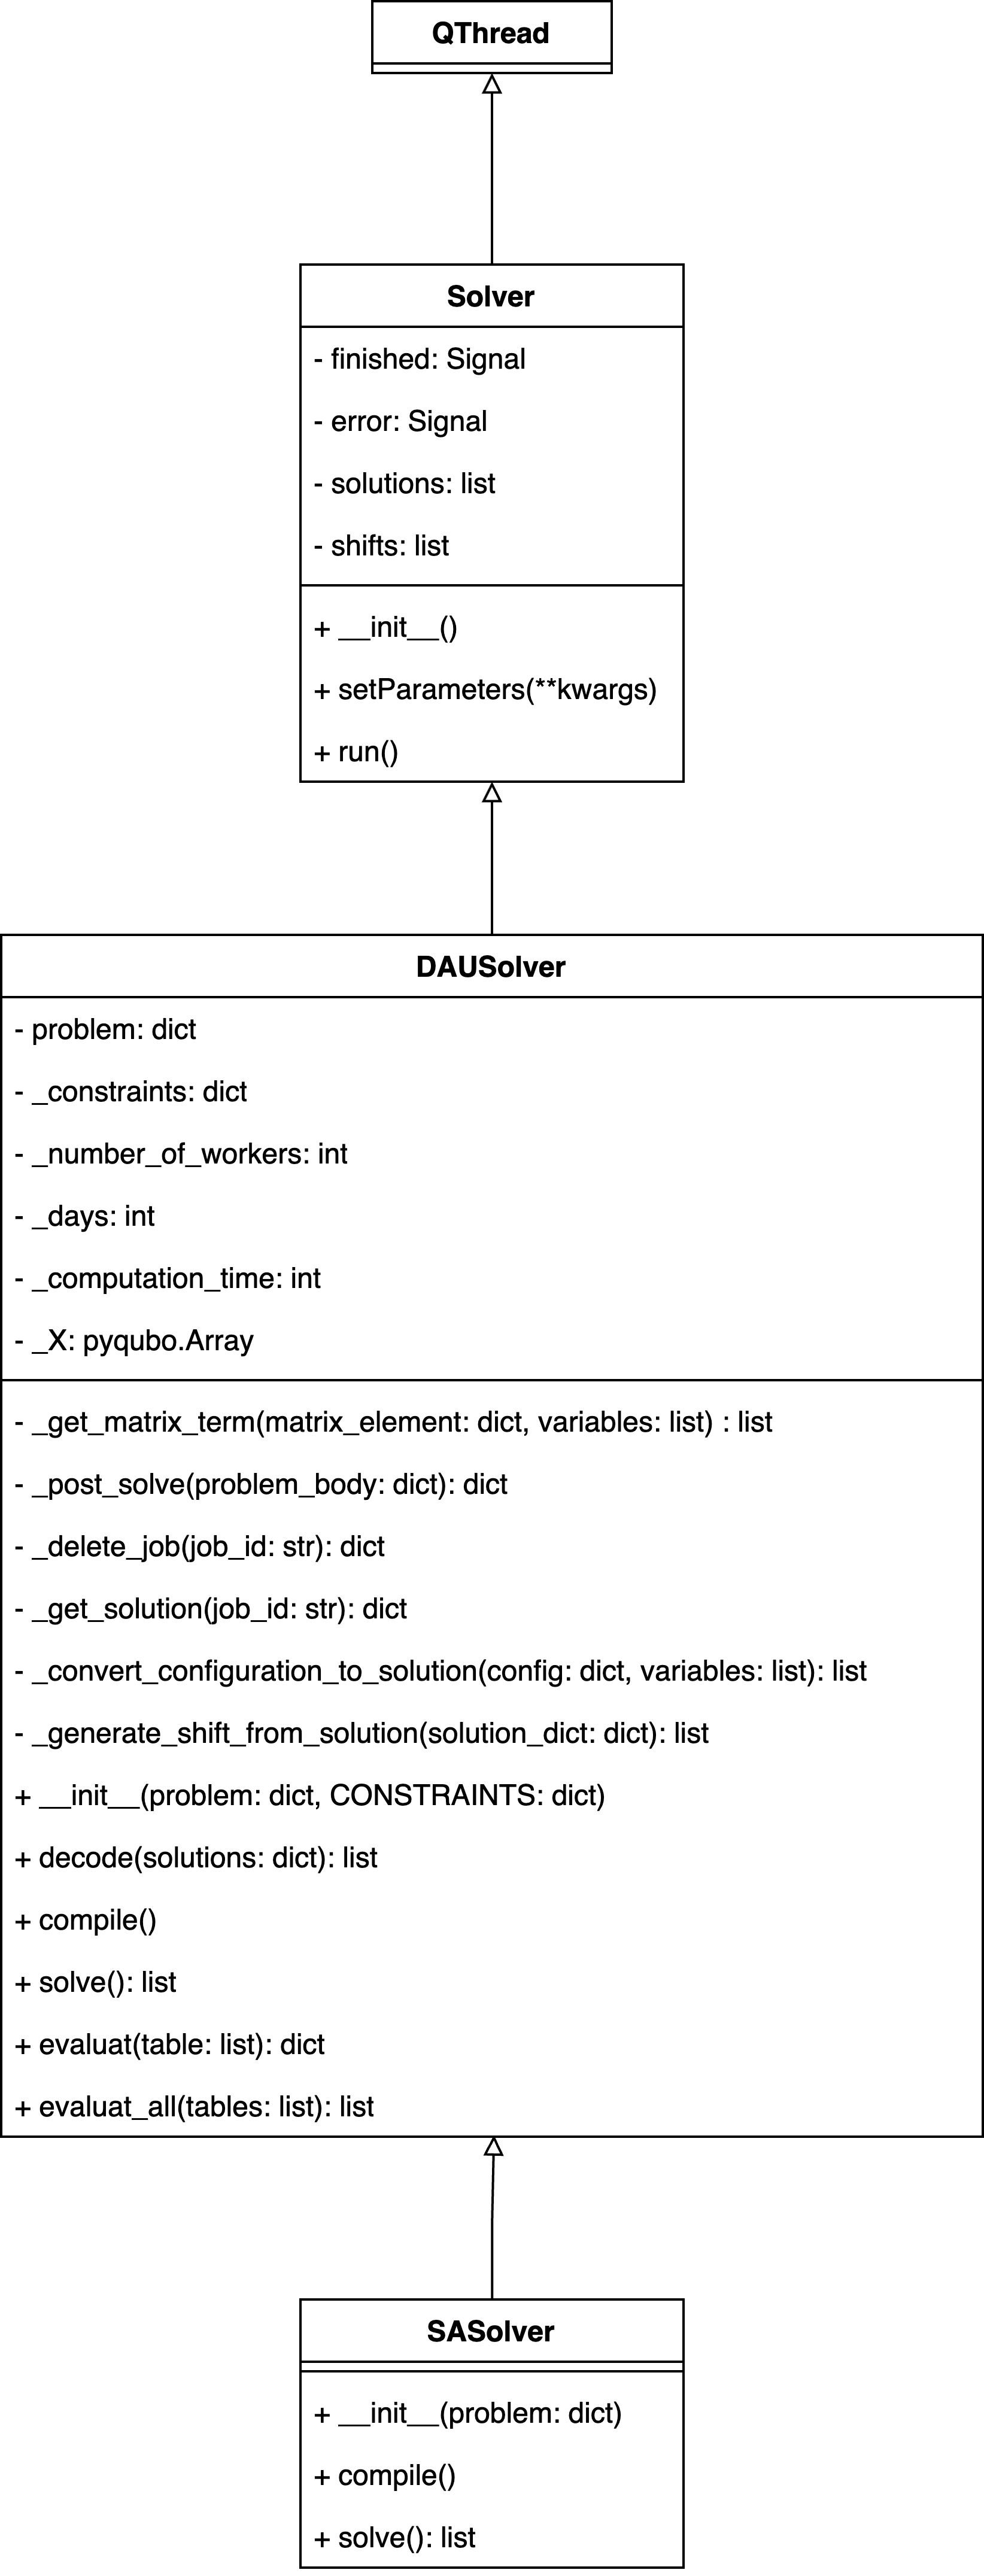
\includegraphics[scale=0.08]{solvers}
\caption{UML of solvers}
\label{umlsolvers}
\end{figure}


\subsubsection{The Expected Number of Working Days}
This requirement could be added to define the number of working days in the shift range. Workers in the shift are expected to have equal working days. The mathematical formulation for $N$ workers and $D$ days shift is as follow:

$$H = \sum_{i}^{N} \left( \sum_{j}^{D}x_{ij} - \alpha \right)^2,
$$
where $\alpha$ is the expected number of working days, and $H$ is the hamiltonian.

\subsubsection{The Expected Number of Workers per Shift}

The following constraint defines the expected number of workers in each shift. This constraint is common and used to balance the workforce and the workload each day. The constraint is modeled by summing up the variables on each shift and minus the expected number of workers and, finally, double themselves and make them quadratic. The mathematical formulation is as follows:(The situation is the same as the one used above)

$$H = \sum_{j}^{D}\left( \sum_{i}^{N} - \beta\right)^2,
$$

where $\beta$ is the expected number of workers each shift.

\subsubsection{Successive Shift Pair}

This constraint is placed to make each worker has at least two consecutive shift. Here's the situation we don't want. The concept is shown below in regular expression form $((0|1)^*0 | 0^*)1(0^* | 0(0|1)^*)$

To be simple, the mathematical formulation separates the boundary situations, $(0|1)^*01$ and $10(0|1)^*$, and the general situation, $(0|1)^*010(0|1)^*$.

\subsubsection{Consecutive 2 days Leave}

This is a soft constraint for days off preference. When this constraint is employed, the algorithm would try to arrange the days off together.

The mathematical formulation is as follows:
$$H = \sum_{i}^N\sum_{j}^{D-1}\left(1-x_{i,j} * x_{i,j+1}\right)$$.

\subsubsection{No Consecutive 2 Days Leave}

This constraint is an opposite version of the above constraint. The mathematical formulation is as follows:
$$H = \sum_{i}^N\sum_{j}^{D-1}\left[(1-x_{i,j}) * (1 - x_{i,j+1})\right]$$.

\iffalse
\subsubsection{Shift Preference}

Workers are able to set up their shift preferences. They can designate which day they want to take a day off or which day they want to work. The algorithm would try to fulfill each worker's requirement.

The mathematical formulation is as follows:
$$H = \sum_{i}^N\sum_{j}^Dx_{ij}-q_{ij}$$
\fi


\subsubsection{The Maximum Consecutive Shifts}

The constraint set up a limit on the maximum number of consecutive shifts. 

This constraint could be modeled by using the supplementary variables. However, this would result in increasing the problem scale. This technique would probably double or triple the number of original variables. Moreover, the solver, Fujitsu's digital annealer, doesn't know the meaning of each variable after compiling the solution into the accepted data; thus, after the annealing process, it would be possible to find a better solution.

The digital annealer computation service offers users to post the inequality.

The inequalities would be an array and append the following inequality.

$$\sum_{j}^{j+\gamma + 1}x_{ij} \leq \gamma, \   \forall i\in[1, N],\  j\in [1, D-\gamma - 1]$$

where $\gamma$ is the maximum consecutive shifts

\subsubsection{Minimum N-days leave within 7 days}

The constraint is for employees' days off welfare. The employees working in graveyard shifts need to have days off in a range.


\subsection{Database}
We design two models, User, Shift, and a data adapter to save and load the models between code and the documents in the MongoDB. The scope of the models is only between the controller and the data adapter. The fields in the model and the fields in the documents are nearly the same, respectively for both models. Please refer to Fig.~\ref{dataadapteruml}. for the UML of data adapter class.
\begin{figure}
\centering
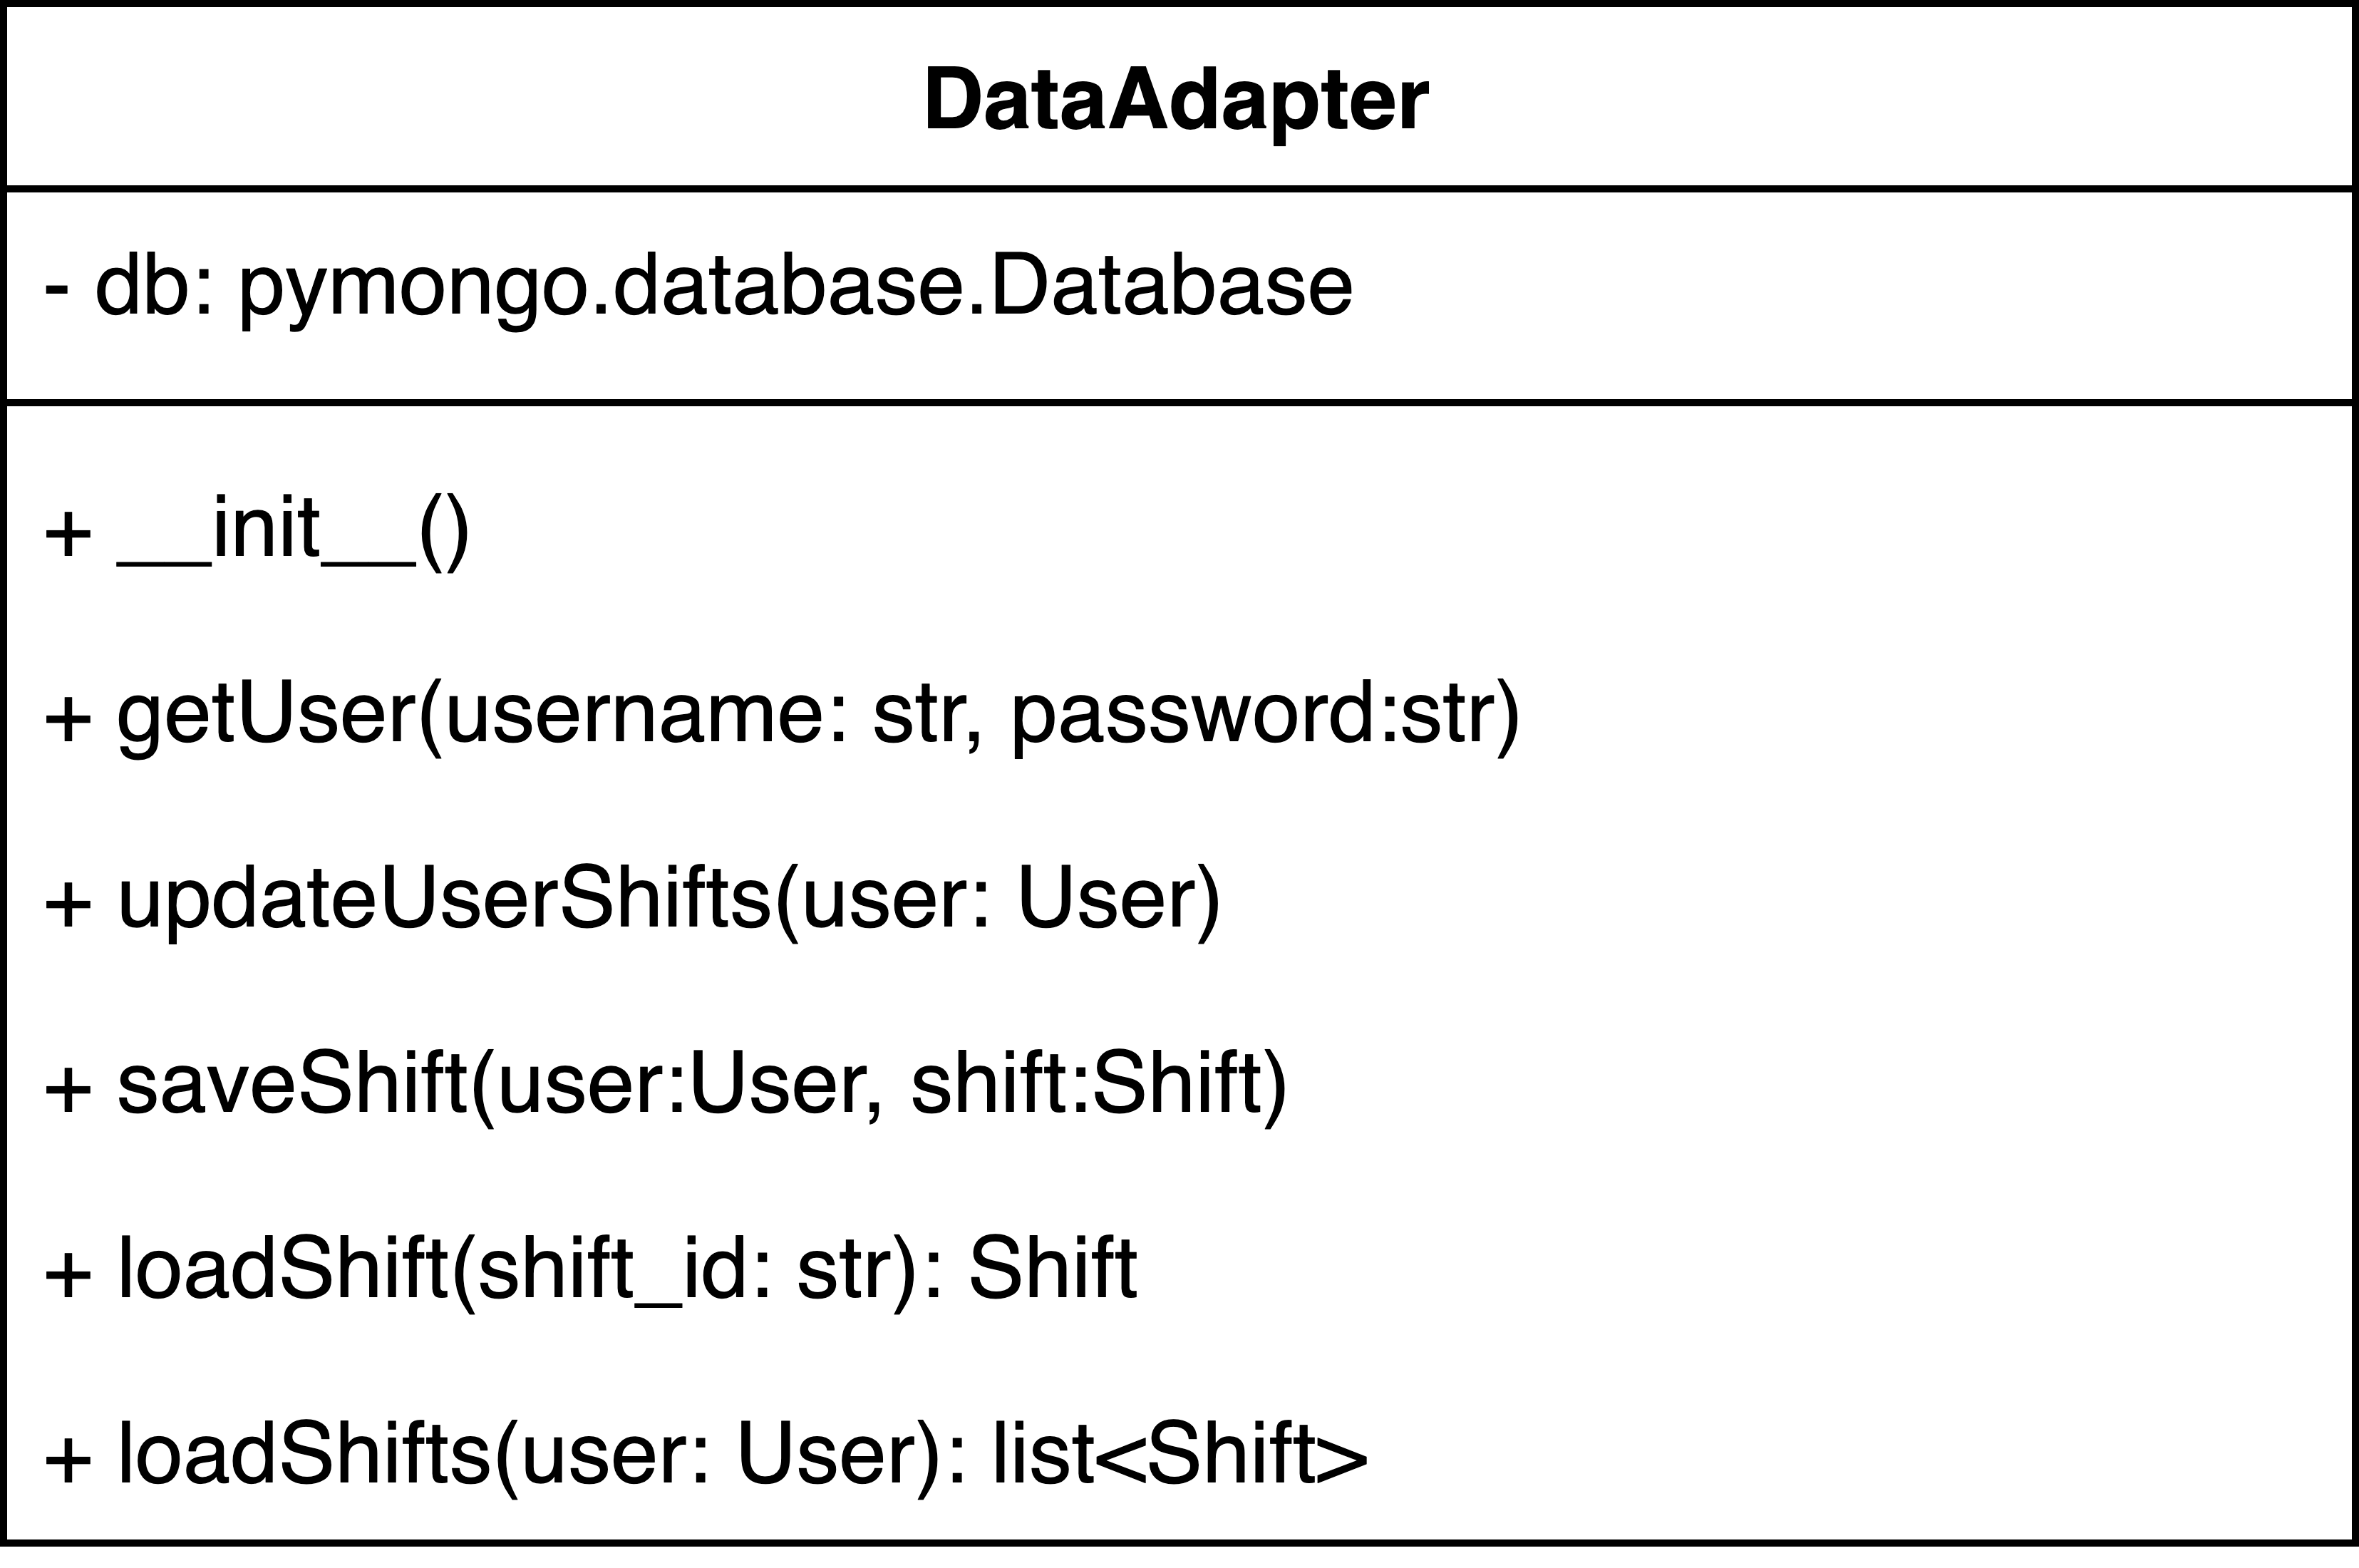
\includegraphics[scale=0.05]{dataadapter}
\caption{Data Adapter UML}
\label{dataadapteruml}
\end{figure}

\section{Runnable Prototype with GUI and Video}
https://youtu.be/uJIEUGbZPPI

\end{document}  